\documentclass{article}
\pdfoutput=1

% \usepackage[utf8]{inputenc}                     % allow utf-8 input
% \usepackage[T1]{fontenc}                        % use 8-bit T1 fonts
\usepackage{hyperref}                           % hyperlinks
\usepackage{url}                                % simple URL typesetting
\usepackage{booktabs}                           % professional-quality tables
\usepackage{amsmath}                            % maths
\usepackage{amsfonts}                           % blackboard math symbols
\usepackage{nicefrac}                           % compact symbols for 1/2, etc.
\usepackage{microtype}                          % microtypography
\usepackage{graphicx}                           % graphs
\usepackage[font=small,labelfont=bf]{caption}   % caption
\usepackage{bbm}                                % indicator
\usepackage{wrapfig}                            % wrap figure
\usepackage{color}                              % color text
\usepackage{fullpage}
\renewcommand{\*}[1]{\textbf{#1}}               % bold
\renewcommand{\u}{$\uparrow$}
\renewcommand{\d}{$\downarrow$}
\renewcommand{\r}[1]{\textcolor{red}{#1}}
\renewcommand{\b}[1]{\textcolor{blue}{#1}}
\setlength{\parindent}{0em}                     % Paragraph spacing.
\setlength{\parskip}{1em}                       % Paragraph spacing.

\title{End-to-End Instance Segmentation and Counting with Recurrent Attention}

\author{
    Mengye Ren \\
    University of Toronto \\
    \texttt{mren@cs.toronto.edu} \\
    \and
    Richard S. Zemel \\
    University of Toronto \\
    Canadian Institute for Advanced Research \\
    \texttt{zemel@cs.toronto.edu} \\
}

\begin{document}
\maketitle
\begin{abstract}
While convolutional neural networks have gained impressive success
recently in solving structured prediction problems such as semantic
segmentation, it remains a
challenge to differentiate individual object instances in the scene.
Instance segmentation is very important
in a variety of applications, such as autonomous driving, image
captioning, and visual question answering.
Techniques that combine large graphical models with low-level vision
have been proposed to address this problem; however, 
We propose an end-to-end recurrent neural network (RNN)
architecture with an attention mechanism to model a 
human-like counting process, and produce detailed instance segmentations. 
The network is jointly trained to sequentially produce regions of
interest as well as a dominant object segmentation within each region. The
proposed model achieves state-of-the-art results on the CVPPP leaf segmentation
dataset \cite{minervini14cvppp} and KITTI vehicle segmentation dataset
\cite{geiger12kitti}.
\end{abstract}

\newcommand{\cvpppAttnImg}[1] {
\includegraphics[width=0.09\textwidth]{./figs/cvppp_internal/plant#1_attn_00_04.png} &
\includegraphics[width=0.09\textwidth]{./figs/cvppp_internal/plant#1_attn_01_04.png} &
\includegraphics[width=0.09\textwidth]{./figs/cvppp_internal/plant#1_attn_02_04.png} &
\includegraphics[width=0.09\textwidth]{./figs/cvppp_internal/plant#1_attn_03_04.png} &
\includegraphics[width=0.09\textwidth]{./figs/cvppp_internal/plant#1_attn_04_04.png} &
\includegraphics[width=0.09\textwidth]{./figs/cvppp_internal/plant#1_attn_05_04.png} &
\includegraphics[width=0.09\textwidth]{./figs/cvppp_internal/plant#1_attn_06_04.png} &
\includegraphics[width=0.09\textwidth]{./figs/cvppp_internal/plant#1_attn_07_04.png} &
\includegraphics[width=0.09\textwidth]{./figs/cvppp_internal/plant#1_attn_08_04.png}}

\newcommand{\cvpppAllImg}[1] {
\includegraphics[width=0.09\textwidth]{./figs/cvppp_internal/plant#1_00.png} &
\includegraphics[width=0.09\textwidth]{./figs/cvppp_internal/plant#1_01.png} &
\includegraphics[width=0.09\textwidth]{./figs/cvppp_internal/plant#1_02.png} &
\includegraphics[width=0.09\textwidth]{./figs/cvppp_internal/plant#1_03.png} &
\includegraphics[width=0.09\textwidth]{./figs/cvppp_internal/plant#1_04.png} &
\includegraphics[width=0.09\textwidth]{./figs/cvppp_internal/plant#1_05.png} &
\includegraphics[width=0.09\textwidth]{./figs/cvppp_internal/plant#1_06.png} &
\includegraphics[width=0.09\textwidth]{./figs/cvppp_internal/plant#1_07.png} &
\includegraphics[width=0.09\textwidth]{./figs/cvppp_internal/plant#1_08.png}}

\begin{figure}
\centering
\resizebox{\columnwidth}{!}{
\begin{tabular}{ccccccccc}
\cvpppAttnImg{045} \\
\cvpppAllImg{045_box} \\
\cvpppAllImg{045_seg_big} \\
\cvpppAllImg{045_total} \\
\end{tabular}
}

\caption{An illustration of outputs of different components of our end-to-end
system, over nine time-steps: Row 1: soft attention  at the current glimpse; 2:
predicted box; 3: current step segmentation; 4: all segmentations. See
\url{https://youtu.be/BMVDhTjEfBU} for a video that shows our our instance
segmentation algorithm in action.}

\end{figure}

\section{Introduction}

Instance segmentation is a fundamental computer vision problem, which aims to
assign pixel-level instance labelling to a given image.  While the standard
semantic segmentation problem entails assigning class labels to each pixel in
an image, it says nothing about the number of instances of each class in the
image. Unlike semantic segmentation, instance segmentation is particularly
difficult in terms of distinguising nearby and occluded objects. Segmenting
at the instance level is useful for many tasks, such as highlighting the
outline of objects for improved recognition and allowing robots to delineate
and grasp individual objects. Obtaining instance level pixel labels is also
significant with respect to general machine understanding of images.

Counting the objects in an image is also of practical value, and is another
problem of interest of this work. Traditionally, counting is performed in a
task-specific setting, either by detection followed by regression, or by
learning discriminatively with a counting distance metric
\cite{lempitsky10count}. Studies in applications such as image question
answering \cite{antol15vqa, ren15vqa} also reveal that counting, especially on
everyday objects, is a very challenging task on its own
\cite{chattopadhyay16count}.

One of the main challenges of instance segmentation is object occlusion.
Classical object detection pipelines \cite{ren15fasterrcnn} is composed of four
stages: proposals, scoring, refinement, and non-maximal suppression (NMS). NMS
typically utilizes a hard threshold that is fixed for the entire dataset. In
cluttered scenes, NMS may suppress the detection results for a heavily occluded
object because it has too much overlap with foreground objects. This challenge
remains in the problem of instance segmentation, which is a more difficult
version of object detection. One motivation of this work is to introduce a way
of performing dynamic NMS to reason about occlusion.

In addition to object occlusion, another challenge is the dimensionality of the
structured output, which is bounded by the number of pixels times the maximum
number of objects. Standard fully convolutional networks (FCN) \cite{long15fcn}
will have trouble directly outputting all instance labels in a single shot.
Recent work on instance segmentation \cite{silberman14insseg,
zhang15insseg,zhang16insseg}  formulates complex graphical models, which
results in a complex and time-consuming pipeline. Furthermore, these models
cannot be trained in an end-to-end fashion.

To tackle both these challenges, we propose a new model based on a recurrent
neural network (RNN) that utilizes visual attention, to perform instance
segmentation.  Our system addresses the dimensionality issue by using a
temporal chain that outputs a single instance at a time. It also performs
dynamic NMS, using an object that is already segmented to aid in the discovery
of an occluded object later in the sequence. Using an RNN to segment one
instance at a time is also inspired by human-like iterative and attentive
counting processes. For real-world cluttered scenes, iterative counting with
attention will likely perform better than a regression model that operates on
the global image level.

In this work, we focus on instance segmentation of a single object-type per
image. We evaluate our model on a number of challenging datasets: 1) CVPPP leaf
segmentation dataset \cite{minervini14cvppp}; 2) KITTI car segmentation dataset
\cite{geiger12kitti}; and 3) on MS-COCO \cite{lin14mscoco} images, where we
train two different models, for ``person'' and ``zebra'' categories, and test
the model with images that contain at least one instance of the chosen
category. We show state-of-the-art performance on both CVPPP and KITTI dataset,
and impressive counting ability on MS-COCO.

\section{Recurrent attention model} 

Our proposed model has four major components: A) a \textbf{2D external memory}
that tracks the state of the segmented objects; B) a \textbf{box proposal network}
responsible for localizing objects of interest;  C) a \textbf{segmentation network} 
for segmenting image pixels within the box; and D) a \textbf{scoring network} 
that determines if an object instance has been found, and also decides when to stop.
See Figure~\ref{fig:model_arch} for an illustration of these components.

\begin{figure}
\begin{center}
\begin{tabular}{cc}
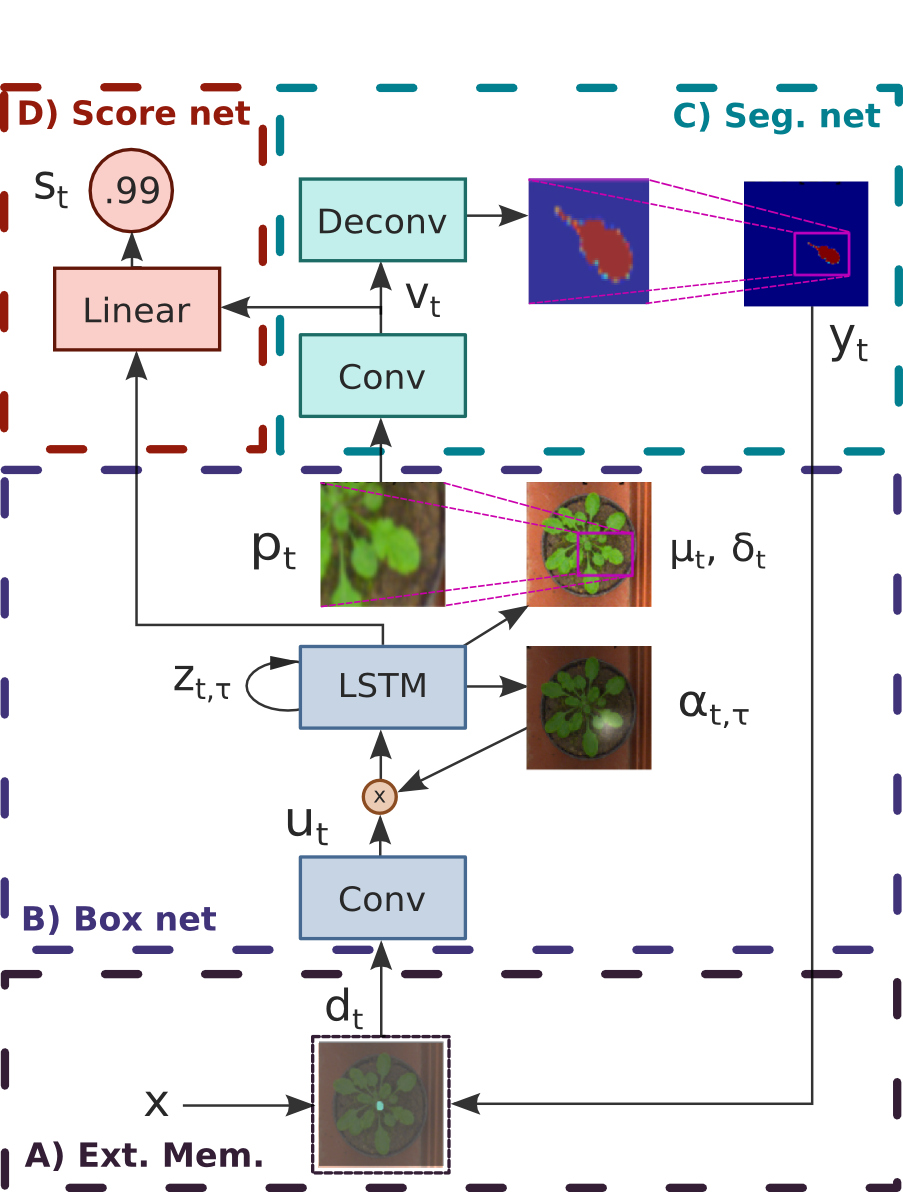
\includegraphics[width=0.52\textwidth]{./figs/model_arch.png} &
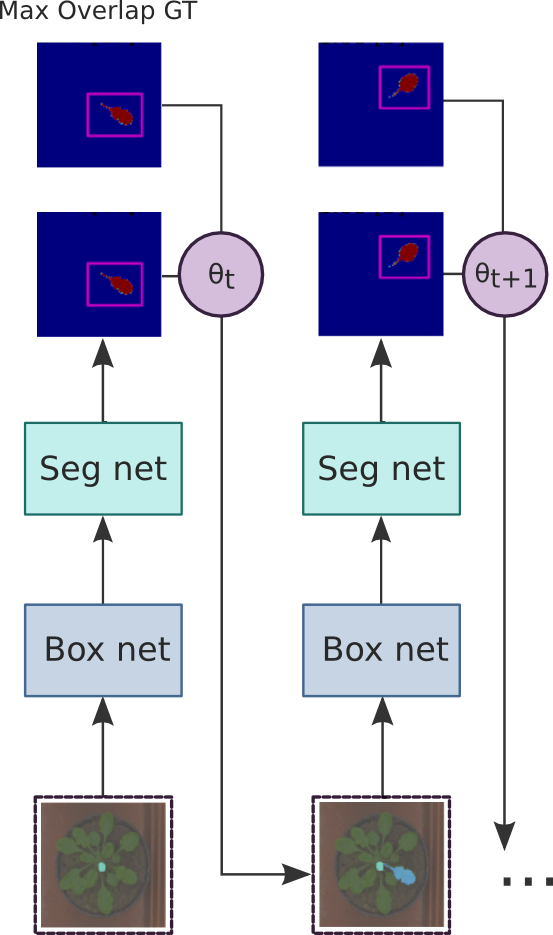
\includegraphics[width=0.38\textwidth]{./figs/model_arch2.png}
\end{tabular}
\end{center}
\caption{
Left: Detailed network design.
Right: Sketch of training, and scheduled sampling;
during training, the weighting of
ground-truth instance segmentations
relative to model predictions
($\theta_t$) decays to zero.
}
\label{fig:model_arch}
\end{figure}


\textbf{Notation}. We use the following notation to describe the model
architecture: $x \in \mathbb{R}^{H \times W}$
is the input image; $y_{t}$, $y^*_{t} \in (0, 1)^{H \times W}$ is the
segmentation  output/ground-truth sequence; $s_{t}$, $s^*_{t} \in (0, 1)$ is
the confidence score output/ground-truth sequence; $\mathcal{W}(z) = w^T z + b$ is a learned
affine transformation.

%%%%%%%%%%%%%%%%%%%%%%%%%%%%%%%%%%%%%%%%%%%%%%%%%%%%%%%%%%%%%%%%%%%%%%%%%%%%%%%
%%%%%%%%%%%%%%%%%%%%%%%%%%%%%%%%%%%%%%%%%%%%%%%%%%%%%%%%%%%%%%%%%%%%%%%%%%%%%%%
\subsection{Part A: Model input and external 2D memory}

We explore three variants of our model which differ in the first component. In
one formulation the input is the raw image, and in the others the image is fed
into a pretrained fully convolutional network (FCN). This \textbf{Pretrained
FCN} has two channels of output.  The first is a pixel-level foreground
segmentation, produced by a variant of the DeconvNet \cite{noh15deconv} with
skip connections. In addition to predicting this foreground mask, as a second
channel we followed the work of Uhrig et al. \cite{uhrig16insseg}  by producing
a 2-d object angle map. For each foreground pixel, we calculate its relative
angle towards the centroid of the object, and quantize the angle into 8
different classes, as shown in Figure~\ref{fig:fcn}. The angle map forces the
model to learn object boundary information, which is missing in the foreground
segmentation.  The architecture and training of these components are detailed
in the Appendix. We denote $D_0(x)$ as the pretrained FCN applied to the
original image.

\begin{figure}
\begin{center}
\resizebox{\columnwidth}{!}{
\begin{tabular}{ccc}
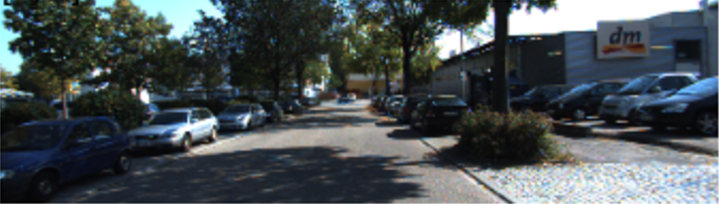
\includegraphics[width=0.5\textwidth]{./figs/fcn_out/fcn_input.png} &
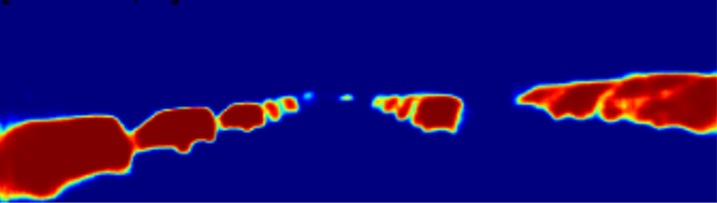
\includegraphics[width=0.5\textwidth]{./figs/fcn_out/fcn_seg.png} &

\includegraphics[width=0.5\textwidth]{./figs/fcn_out/fcn_angle.png}
\end{tabular}
}
\caption{Illustration of the output of the pretrained FCN. Left: input image.
Middle: predicted foreground. Right: predicted angle map.}
\label{fig:fcn}
\end{center}
\end{figure}


To facilitate learning to sequentially enumerate the objects, we incorporate an
external 2D memory in the RNN structure. We treat this 2D memory as the third
channel of the model input. We explore two alternative formulations of this
memory: 1) a \textbf{cumulative canvas} that stores the full history of
segmentation outputs, and 2) a \textbf{convolutional-RNN} with extra parameters
to dynamically adapt memory storage. Both operate at the full input resolution
to precisely deal with occlusion.

1. \textbf{\textit{Cumulative canvas}}. We hypothesize that providing
information of the completed segmentation helps the network reason about
occluded objects and determine the next region of interest. The first channel of
the canvas keeps adding new pixels from the output of the previous time step.
\vspace{-1pt}
\begin{align}
d_t^{\text{Canvas}} = \left[c_{t}, D_0(x)\right], \ \ \ \ 
c_0^{\text{Canvas}} &= 0, \ \ \ \
c_t^{\text{Canvas}} = \max(c_{t-1}, y_{t-1}) \ \forall t > 0
\end{align}
\vspace{-4pt}

2. \textbf{\textit{Convolutional LSTM}}. One issue of the cumulative canvas is
that the recurrent connection from the output of the previous time step into
the canvas sometimes leads to training instability. In practice, we observe
that reducing the gradient flowing back from the input of the canvas  aids
training. An alternative is to learn the ``addition'' operation with another
RNN. Convolutional LSTM \cite{shi2015convlstm} is a form of RNN that uses
convolution as its recurrent operator and thus is able to efficiently process
a 2D image input and store a 2D hidden state. We initialize the hidden state of
the ConvLSTM with the FCN output, and feed the output segmentation back
into the ConvLSTM (See Figure~\ref{fig:model_arch}, right). This allows the
gradient to flow through the ConvLSTM without introducing instability.
\vspace{-1pt}
\begin{align}
d_0^{\text{ConvLSTM}} &= D_0(x),\ \ \ \ 
d_{t}^{\text{ConvLSTM}} = \text{ConvLSTM}(d_{t-1}, y_{t-1}) \ \forall t > 0
\end{align}
\vspace{-6pt}

%%%%%%%%%%%%%%%%%%%%%%%%%%%%%%%%%%%%%%%%%%%%%%%%%%%%%%%%%%%%%%%%%%%%%%%%%%%%%%%
%%%%%%%%%%%%%%%%%%%%%%%%%%%%%%%%%%%%%%%%%%%%%%%%%%%%%%%%%%%%%%%%%%%%%%%%%%%%%%%
\subsection{Part B: Box network}

The box network localizes objects of interest. The CNN in the box network
outputs a $H' \times W' \times L$ feature map $u_{\text{box}, t}$. We employ a
``soft-attention'' mechanism here to extract useful information along spatial
dimensions and feed a dimension $L$ vector into the glimpse LSTM. Since one
single glimpse may not give the upper network enough information to decide
where exactly to draw the box, we allow the glimpse LSTM to look at different
locations.  $\alpha$ is  initialized to be uniform over all locations, and
$\tau$ indexes the glimpses.
\vspace{-1pt}
\begin{align}
u_{\text{box},t} = \text{CNN}(d_t), \ \ \ \
z_{t, \tau} &= \text{LSTM} (
\sum_{h, w} \alpha^{h, w}_{t, \tau} u^{h,w,l}_{\text{box},t}, z_{t, \tau-1} ), \ \ \ \
\alpha_{t, \tau+1} = \text{MLP}(z_{t, \tau})
\end{align}
\vspace{-6pt}

We pass the LSTM's hidden state through a linear layer to obtain predicted
box coordinates. We parameterize the box by its normalized center
$g_{X,Y}$, and log size $\log \delta_{X,Y}$. A scaling factor $\gamma$ is
also predicted by the linear layer, and used when re-projecting the patch
to the original image size.
\vspace{-1pt}
\begin{align}
(\tilde{g}_{X,Y}, \log \tilde{\delta}_{X,Y}, \log \sigma_{X,Y}, \gamma) &= \mathcal{W}(z_{t, \text{end}})
\end{align}
\begin{align}
g_X, g_Y &= (\tilde{g}_X+1)\frac{W}{2}, (\tilde{g}_Y+1)\frac{H}{2}, \ \ \ \  
\delta_X, \delta_Y = \tilde{\delta}_X W, \tilde{\delta}_Y H
\end{align}
\vspace{-6pt}

\textbf{Extracting a sub-region}. We follow DRAW \cite{gregor15draw} and use a
Gaussian interpolation kernel to extract a patch from the $\tilde{x}$, a
concatenation of the original image with $d_t$. We further allow the model to
output rectangular patches to account for different shapes of the object.
\begin{align}
\mu_X^i, \mu_Y^j &= g_X + (\delta_X + 1) \cdot (i - N / 2 + 0.5) / N, \ \  
g_Y + (\delta_Y + 1) \cdot (j - N / 2 + 0.5) / N
\end{align}
\begin{align}
F_X[a, i], F_Y[b, j] &= 
\frac{1}{\sqrt{2\pi} \sigma_X} \exp \left(- \frac{(a -
\mu_X^i)^2}{2\sigma_X^2} \right), 
\frac{1}{\sqrt{2\pi} \sigma_Y} \exp \left(- \frac{(b -
\mu_Y^j)^2}{2\sigma_Y^2} \right)
\end{align}
\begin{align}
p_t &= \text{Extract}(\tilde{x}_t, F_Y, F_X) \equiv F_Y^T \tilde{x}_t F_X
\end{align}
%\vspace{-6pt}

%%%%%%%%%%%%%%%%%%%%%%%%%%%%%%%%%%%%%%%%%%%%%%%%%%%%%%%%%%%%%%%%%%%%%%%%%%%%%%%
%%%%%%%%%%%%%%%%%%%%%%%%%%%%%%%%%%%%%%%%%%%%%%%%%%%%%%%%%%%%%%%%%%%%%%%%%%%%%%%
\subsection{Part C: Segmentation network}

The remaining task is to segment out the pixels that belong to the dominant
object within the window. In the segmentation network, we adopt a variant of
the DeconvNet \cite{noh15deconv} with skip connections, which appends
deconvolution (or convolution transpose) layers after convolution layers to
upsample the low-resolution feature map to a full-size segmentation. After the
fully convolutional layers, we get a patch-level segmentation prediction heat
map $\tilde{y}_t$. We then re-project this patch prediction to the original
image using the transpose of the previous computed Gaussian filters. The
learned $\gamma$ to magnifies the signal within the bounding box, and a
constant $\beta$ to suppresses the pixels outside the box. Lastly, the sigmoid
function produces final segmentation values between 0 and 1.
\begin{align}
y_t &= \text{sigmoid} \left(
\gamma \cdot \text{Extract}(\tilde{y}_t, F_Y^T, F_X^T)
- \beta \right)
\end{align}
%\vspace{-6pt}

%%%%%%%%%%%%%%%%%%%%%%%%%%%%%%%%%%%%%%%%%%%%%%%%%%%%%%%%%%%%%%%%%%%%%%%%%%%%%%%
%%%%%%%%%%%%%%%%%%%%%%%%%%%%%%%%%%%%%%%%%%%%%%%%%%%%%%%%%%%%%%%%%%%%%%%%%%%%%%%
\subsection{Part D: Scoring network}

To estimate the number of objects in the image, and to terminate our sequential
process, we incorporate a scoring network, similar to the one presented in
\cite{romeraparedes15ris}. Our scoring network takes information from the box
and segmentation network to produce a score between 0 and 1.
\begin{equation}
s_{t} = \text{sigmoid}(\mathcal{W}(z_{t, \text{end}}) + \mathcal{W}(u_{\text{segm}}))
\end{equation}
%\vspace{-4pt}

\textbf{Termination condition}. We train the entire model with a sequence length
determined by the maximum number of objects plus one. During inference, we cut
off iterations once the output score goes below 0.5. The loss function
(described below) encourages scores to decrease monotonically.
%\vspace{-4pt}

%%%%%%%%%%%%%%%%%%%%%%%%%%%%%%%%%%%%%%%%%%%%%%%%%%%%%%%%%%%%%%%%%%%%%%%%%%%%%%%
%%%%%%%%%%%%%%%%%%%%%%%%%%%%%%%%%%%%%%%%%%%%%%%%%%%%%%%%%%%%%%%%%%%%%%%%%%%%%%%
\subsection{Loss functions}

\textbf{Joint loss}. The total loss function is a sum of three losses:
the segmentation matching IoU loss $L_y$; the box IoU loss $L_b$;
and the score cross-entropy loss $L_s$:
\vspace{-3pt}
\begin{equation}
L(y, b, s) = L_y(y, y^*) + L_b(b, b^*) + L_s(s, s^*)
\end{equation}
\vspace{-4pt}

\textbf{(a) Matching IoU loss (mIOU)}. A primary challenge of instance segmentation
involves matching model and ground-truth instances.  we compute a
maximum-weighted 
bipartite graph matching between the output instances and ground-truth
instances \cite{stewart15lstmdet} and \cite{romeraparedes15ris}. Matching makes
the loss insensitive to the ordering of the ground-truth instances. Unlike
coverage scores proposed in \cite{silberman14insseg} it directly penalizes both
false positive and false negative segmentation. The matching weight $M_{i, j}$
is the IoU score between a pair of segmentation. We use the Hungarian algorithm
to compute the matching.
%\vspace{-3pt}
\begin{align}
M_{i, j} &= \text{softIOU}(y_i, y^*_j) \equiv \frac{\sum y_i \cdot y^*_j}
{\sum y_i + y^*_j - y_i \cdot y^*_j} \\
L_y(y, y^*) &= -\text{mIOU}(y, y^*) \equiv -\frac{1}{N} \sum_{i, j} 
M_{i, j} \mathbbm{1}[\text{match}(y_i) = y^*_j]
\end{align}
%\vspace{-12pt}

\textbf{(b) Soft box IoU loss}. Although the exact IoU can be derived from the 4-d
box coordinates, its gradient vanishes when two boxes do not overlap, which can
be problematic for gradient-based  learning. Instead, we propose a soft version
of the box IoU. We use the same Gaussian filter to re-project a constant patch
on the original image, pad the ground-truth boxes and compute the mIOU between
the predicted box and the matched padded ground-truth bounding box.
\vspace{-3pt}
\begin{align}
b_{t} &= \text{sigmoid}(\gamma \cdot \text{Extract}(\mathbf{1}, F_Y^T, F_X^T) -
\beta)\\
L_b(b, b^*) &= -\text{mIOU}(b, \text{Pad}(b^*))
\end{align}
%\vspace{-12pt}

\textbf{(c) Monotonic score loss}. To facilitate automatic termination, the
network should output more confident objects first. We proposed a loss function
that encourages monotonically decreasing values in the score output. Iterations
with target score 1 are compared to the lower bound of preceding scores, and 0
targets to the upper bound of subsequent scores.
\vspace{-3pt}
\begin{align}
L_s(s, s^*) &= \sum_t -s^*_t 
\log\left(\max_{t'=t...T-1} \{s_{t'}\}\right) - (1 - s^*_t)
\log\left(1 - \min_{t'=0...t} \{s_{t'}\}\right)
\end{align}
%\vspace{-12pt}

%%%%%%%%%%%%%%%%%%%%%%%%%%%%%%%%%%%%%%%%%%%%%%%%%%%%%%%%%%%%%%%%%%%%%%%%%%%%%%%
%%%%%%%%%%%%%%%%%%%%%%%%%%%%%%%%%%%%%%%%%%%%%%%%%%%%%%%%%%%%%%%%%%%%%%%%%%%%%%%
\subsection{Training procedure and post-processing}
\vspace{-3pt}

\textbf{Bootstrap training}. The box and segmentation networks rely on the
output of each other to make decisions for the next time-step. Because of the
coupled nature of the two networks, we propose a bootstrap training procedure:
these networks are pre-trained with ground-truth segmentation and boxes, 
respectively, and in later stages we replace the ground-truth with the model 
predicted values.

\textbf{Scheduled sampling}. To smooth out the transition between stages, we
explore the idea of ``scheduled sampling'' \cite{bengio15schedsamp} where we
gradually remove the reliance on ground-truth segmentation at the input of the
network. As shown in Figure~\ref{fig:model_arch}, during training there
is a dynamic switch in the input of the external memory, to utilize either the
maximally overlapping ground-truth instance segmentation, or the 
output of the network from the previous time step.

We denote $\theta_t$ as the probability of feeding in ground-truth segmentation
that has the greatest overlap with the previous prediction. $\theta_t$ follows
exponential decay as training goes on, and for larger $t$, the decays comes in
later.
\vspace{-3pt}
\begin{align}
\theta_t &= 
\min \left(\Gamma_t \exp \left(-\frac{step - S}{S_2} \right), 1 \right) \\
\Gamma_t &= 1 + \log(1 + Kt)
\end{align}

\textbf{Post-processing}. We truncate segmentation outside the predicted
foreground mask, fill holes with the labels from the nearest neighboring
predicted instance, and remove object segmentation of size smaller than 425
square pixels. We study the effect of post-processing in ablation studies in
Table~\ref{tab:kitti}.

\section{Related Work}

Instance segmentation has recently received a burst of research attention, as
it provides higher level of precision of image understanding compared to object
detection and semantic segmentation.

\textbf{Instance segmentation using graphical models}. An early exploration of
instance segmentation proposes a multi-stage pipeline composed of patch-wise
features based on deep learning, combined into a segmentation tree
\cite{silberman14insseg}. They formulated a new loss function, the coverage
score, that calculated the amount of ground truth regions not covered by the
model's instance segmentation. More recently, Zhang et al. \cite{zhang16insseg}
formulated a dense CRF for instance segmentation; .  They apply a CNN on dense
image patches to make local predictions, and constructed a dense CRF to produce
globally consistent labellings. Their key contribution is a shifting-label
potential that encourages consistency across different patches. They achieved
strong results on the challenging KITTI object dataset; however, the graphical
model formulation entails long running times, and their energy functions are
dependent on instances being connected and having a clear depth ordering.

\textbf{Instance segmentation using CNN}. Liang et al.~\cite{liang15pfinsseg}
used a CNN to generate pixel-level object size information, and used clustering
as a post-processing step. They added a regressor at the top of the CNN to
estimate the count, which is the total number of clusters. An erroneous count
can usually leads to poor segmentation. Dai et al.~\cite{dai15insaware}
proposed a pipeline-based approach and won the MS-COCO instance segmentation
challenge. Their method first predicts bounding box proposals and extracts
regions of interest (ROI), then uses shared features to perform segmentation
within each ROI. Their architecture can also be fine-tuned end-to-end. However,
since their method is based on detector proposals, it does not explicitly
handle object occlusions, which may lead it to fail during  non- maximal
suppression (NMS). Uhrig et al.~\cite{uhrig16insseg} presented another approach
with FCN, and achieved very impressive results. Their FCN outputs three
channels: semantic segmentation, object orientation and depth. Post-processing
based on template matching and instance fusion produce the instance identities.
Their approach is based on bottom-up clustering since their FCN can only
provide pixel-level information, whereas our model is processing the image in a
top-down fashion. Importantly, they also used ground-truth depth labels in
training their model.

\textbf{Instance segmentation using RNN}. Other recent line of research, e.g.
\cite{stewart15lstmdet, park15ris, romeraparedes15ris} employs end-to-end
recurrent neural networks (RNN) to perform object detection and segmentation. A
permutation agnostic loss function based on maximum weighted bipartite matching
was proposed by \cite{stewart15lstmdet}. To process an entire image, they treat
each element of a $15\times20$ feature map individually. Similarly, our box
proposal network also uses an RNN to generate box proposals: instead of running
the image 300 times through the RNN, we only run it once by using a soft
attention mechanism \cite{xu15caption}. Romera-Paredes and Torr
\cite{romeraparedes15ris} use convolutional LSTM (ConvLSTM)
\cite{shi2015convlstm} to produce instance segmentation directly. However,
since their ConvLSTM is required to handle object detection, inhibition, and
segmentation all at the same time on a global scale, the final output loses
precision. They add a dense CRF to restore the resolution. Compared to their
approach, our segmentation network operates on a local level. Instead of
resorting to graphical models, we added skip connections to restore the
resolution.

\textbf{Instance counting}. Previous work on object counting in images has
mainly focused on pedestrians crowd and biological cells
\cite{lempitsky10count}. Chattopadhyay et al. \cite{chattopadhyay16count}
focused on counting questions in VQA and proposed detector approaches as well
as a regression based method (``associative subitizing'') that works on a $3
\times 3$ field of CNN features level. Note that unlike our approach, this
method does not provide instance segmentations.

\section{Experiments}

\textbf{CVPPP leaf segmentation}. One instance segmentation benchmark is the
CVPPP plant leaf dataset \cite{minervini14cvppp}, which was developed due to
the importance of instance segmentation in plant phenotyping. We ran the A1
subset of CVPPP plant leaf segmentation dataset. We trained our model on 128
labelled images, and report results on the 33 test images. We compare our
performance to \cite{romeraparedes15ris}, and other top approaches that were
published with the CVPPP conference; see the collation study
\cite{scharr16leaf} for details of these  other approaches.

\textbf{KITTI car segmentation}. Instance segmentation also provides rich
information in the context of autonomous driving. Following
\cite{zhang15insseg, zhang16insseg, uhrig16insseg}, we also evaluated the model
performance on KITTI car segmentation dataset. We trained the model with 3712
training images, and report performance on 144 test images. We also examine the
relative importance of model components via ablation studies.

\textbf{MS-COCO counting}. Additionally, we train class specific models on
MS-COCO and test counting performance on the results. We chose ``person'' and
``zebra'' because these are the two of the most common classes in VQA
questions. We report counting performance on images with at least one instance
of the class: 677 zebra images, and 21,634 ``person'' images.

\begin{table}
\begin{minipage}[t]{.48\textwidth}
% \begin{minipage}[t]{1.0\textwidth}
\caption{Leaf segmentation and counting performance}
\label{tab:cvppp}
\centering
\begin{small}

% \resizebox{1.0\columnwidth}{!}{
\begin{tabular}{l|ll}
\toprule
\toprule
                                  & \*{SBD} \u     & \*{|DiC|} \d    \\
\midrule
RIS+CRF \cite{romeraparedes15ris} & 66.6 (8.7)     & 1.1 (0.9)       \\
MSU \cite{scharr16leaf}           & 66.7 (7.6)     & 2.3 (1.6)       \\
Nottingham \cite{scharr16leaf}    & 68.3 (6.3)     & 3.8 (2.0)       \\
Wageningen \cite{yin14leaf}       & 71.1 (6.2)     & 2.2 (1.6)       \\
IPK \cite{pape14ipk}              & 74.4 (4.3)     & 2.6 (1.8)       \\
PRIAn \cite{giuffrida15count}     & -              & 1.3(1.2)        \\
\midrule
Ours (FCN + Canvas)               & 79.3 (9.2)     & 0.9 (1.0)       \\
Ours (FCN + ConvLSTM)             & 80.4 (8.9)     & 1.0 (0.8)       \\
Ours (Canvas)                     & \*{84.9} (4.8) & \*{0.8} (1.0)   \\
\bottomrule
\end{tabular}
% }
\end{small}
% \end{table}
% }
\end{minipage}
\qquad
\begin{minipage}[t]{.48\textwidth}
\label{tab:vqa}
\caption{Counting performance on MS-COCO}
\centering
\begin{small}
\begin{tabular}{l|lll}
\toprule
\toprule
                                     & \*{Category} & \*{MWCov} \u  & \*{|DiC|} \d \\
\midrule
detect \cite{chattopadhyay16count}   & Person       & -             & 3.22     \\
aso-sub \cite{chattopadhyay16count}  & Person       & -             & \*{1.36} \\
\midrule
Ours                                 & Person       & 48.3          & 2.09     \\
\midrule
\midrule
detect \cite{chattopadhyay16count}   & Zebra        & -             & 2.56     \\
aso-sub \cite{chattopadhyay16count}  & Zebra        & -             & 1.03     \\
\midrule
Ours                                 & Zebra        & 65.3          & \*{0.85} \\
\bottomrule
\end{tabular}
\end{small}
\end{minipage}
\end{table}

\newcommand{\cvpppImg}[1] {
\includegraphics[width=0.133\textwidth]{./figs/cvppp_img/plant#1_rgb.png} &
\includegraphics[width=0.133\textwidth]{./figs/cvppp_gt/plant#1_label.png} &
\includegraphics[width=0.133\textwidth]{./figs/cvppp_out/plant#1_label.png}}

\begin{figure}
\centering
\begin{small}
\resizebox{\columnwidth}{!}{
\begin{tabular}{ccccccc}
Image & GT & Ours & & Image & GT & Ours \\
\cvpppImg{029} & & \cvpppImg{137}\\
\\
\cvpppImg{042} & & \cvpppImg{119}
\end{tabular}
}
\caption{Examples of our instance segmentation output on CVPPP leaf dataset.
In this paper, instance colors are determined by the order of the model output
sequence.}
\label{fig:cvppp_out}
\end{small}
\end{figure}

\begin{table}[t]
\caption{KITTI vehicle segmentation results}
\label{tab:kitti}
\centering
\begin{small}
\begin{tabular}{l|llllll}
\toprule
\toprule
                                 & \*{FG IoU} \u & \*{MWCov} \u & \*{MUCov} \u & \*{AvgFP} \d & \*{AvgFN} \d \\
\midrule
No Sched. Samp.                  & 87.6          & 78.1         & 62.9         & 0.139        & 0.361        \\
No Post Proc.                    & 83.0          & 78.7         & 65.8         & 0.222        & 0.431        \\
\midrule    
DenseCRFv1 \cite{zhang15insseg}  & 77.3          & 70.9         & 52.2         & 0.597        & 0.736        \\
DenseCRFv2 \cite{zhang16insseg}  & 78.5          & 74.1         & 55.2         & 0.417        & 0.833        \\
FCN+Depth \cite{uhrig16insseg}   & 84.1          & 79.7         & \*{75.8}     & 0.201        & \*{0.159}    \\
\midrule
Ours (Canvas)                    & 86.9          & 72.2         & 59.4         & \*{0.090}    & 0.438        \\
Ours (FCN + Canvas)              & \*{86.8}      & 81.0         & 66.6         & 0.167        & 0.396        \\
Ours (FCN + ConvLSTM)            & \*{86.8}      & \*{82.2}     & 67.7         & 0.188        & 0.382        \\
\bottomrule
\end{tabular}
\end{small}
\end{table}

\newcommand{\kittiImg}[1] {
\includegraphics[width=0.3\textwidth]{./figs/kitti_img/#1.png} &
\includegraphics[width=0.3\textwidth]{./figs/kitti_gt/#1.png} &
\includegraphics[width=0.3\textwidth]{./figs/kitti_out/#1.png}}

\begin{figure}
\centering
\begin{small}
\resizebox{\columnwidth}{!}{
\begin{tabular}{ccc}
Image & GT & Ours \\
\kittiImg{002142} \\
\\
\kittiImg{001415} \\
\\
\kittiImg{005057} \\
\\
\kittiImg{004369} \\
\end{tabular}
}
\caption{Examples of our instance segmentation output on KITTI}
\label{fig:kitti_out}
\end{small}
\end{figure}

\begin{figure}[h]
% \begin{wrapfigure}{rt}{0.5\textwidth}
\centering
% \resizebox{0.45\textwidth}{!}{
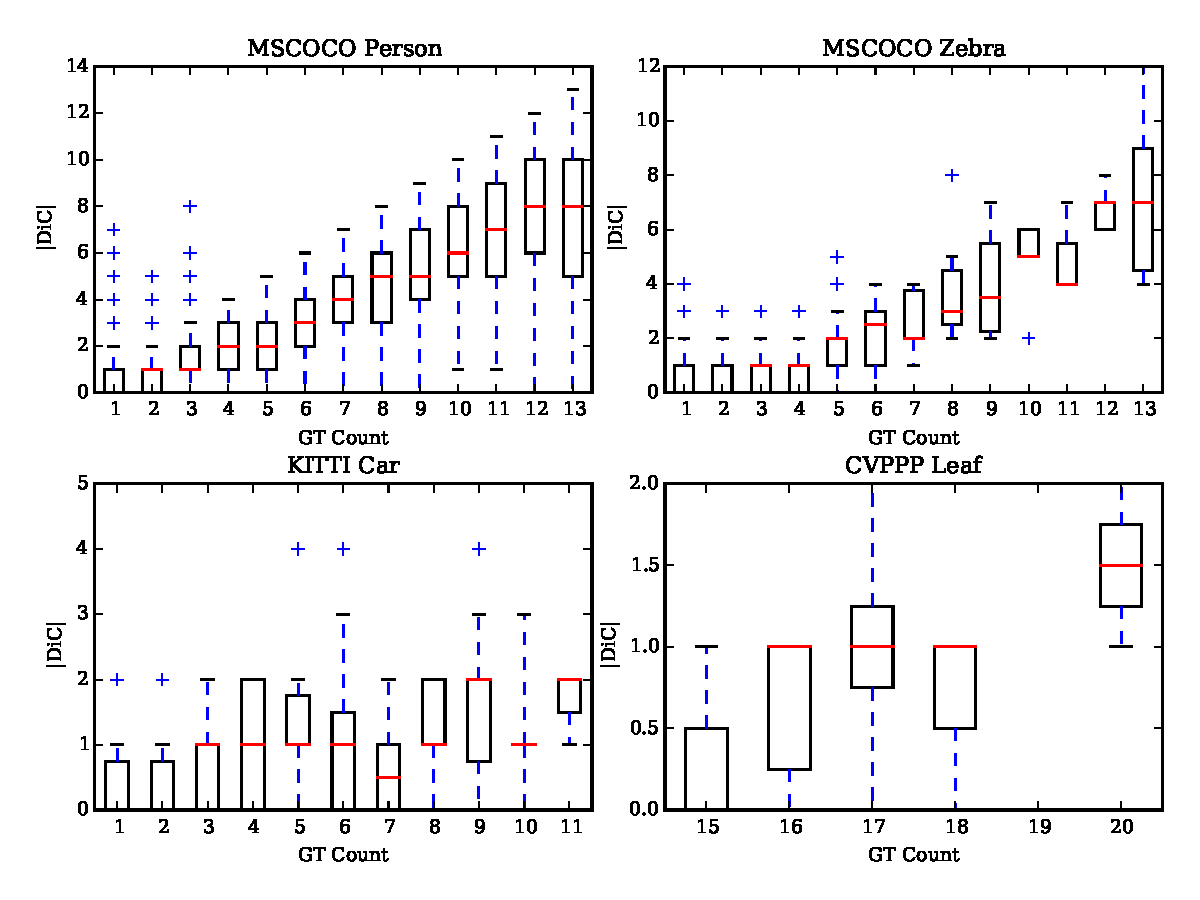
\includegraphics[width=0.8\textwidth]{count.pdf}
\caption{Absolute difference in count between the model and ground-truth as 
a function of the number of objects, in the various datasets.}
\label{fig:count}
% }
% \end{wrapfigure}
\end{figure}


\textbf{Evaluation metrics}. We report the  metrics used by the other studies
in the respective benchmarks: symmetric best dice (SBD) for leaf segmentation
(see Equations~\ref{eq:bd}, \ref{eq:sbd}) and mean (weighted) coverage (MWCov,
MUCov) for car segmentation (see Equations~\ref{eq:mwcov}, \ref{eq:mucov}). The
coverage scores measure the instance-wise IoU for each ground-truth instance
averaged over the image; MWCov further weights the score by the size of the
ground-truth instance segmentation (larger objects get larger weights).
%\vspace{-3pt}

\begin{align}
\label{eq:bd}
\text{DICE}(A, B) &= \frac{2 |A \cup B|}{|A| + |B|} \ \ \ \ \ \ \ \
\text{BD}(\{A_i\}, B) = \max_{i} \text{DICE}(A_i, B) \\
\label{eq:sbd}
\text{SBD}(\{\hat{y}_i\}, \{y_j\}) &= 
\min \left(\frac{1}{N} \sum_j \text{BD}(\{\hat{y}_i\}, y_j), \frac{1}{N}
\sum_i \text{BD}(\hat{y}_i, \{y_j\}) \right)
\end{align}
\vspace{-12pt}
\begin{align}
\label{eq:mwcov}
\text{MWCov}(\{y_i\}, \{y_j^*\}) &= \frac{1}{N} \sum_i 
\frac{|y_i|}{\sum_i |y_i|} \max_j
\text{IoU}(y_i, y_j^*)\\
\label{eq:mucov}
\text{MUCov}(\{y_i\}, \{y_j^*\}) &= \frac{1}{N} \sum_i 
\max_j \text{IoU}(y_i, y_j^*)
\end{align}

Counting is measured in absolute difference in count (|DiC|) (see
Equation~\ref{eq:dic}), average false positive (AvgFP), and average false
negative (AvgFN). False positive is the number of predicted instances that do
not overlap with the ground-truth, and false negative is the number of 
ground-truth instances that do not overlap with the prediction.
\vspace{-3pt}
\begin{align}
\label{eq:dic}
|DiC| = \frac{1}{N}\sum_i |count_i - count_i^*|
\end{align}
\vspace{-12pt}

\subsection{Results \& discussion}
\vspace{-3pt}
In the leaf segmentation task, our best model outperforms the previous 
state-of-the-art by a large margin in both segmentation and counting.
Table~\ref{tab:cvppp} shows that the models with FCN overfit and 
scores lower than the simpler version. This is sensible as the dataset size
is small, and including the FCN significantly increases the input dimension and
number of parameters.

In the car segmentation task, our model achieves the state-of-the-art MWCov
shown in Table~\ref{tab:kitti}, but our MUCov is lower than results reported by
Uhrig et al. \cite{uhrig16insseg}. One possible explanation is their inclusion
of depth information during training, which may help the model disambiguate
distant object boundaries. Moreover, their bottom-up ``instance fusion'' method
plays a crucial role (omitting this leads to a steep performance drop); this
likely helps segment smaller objects, whereas our box network does not reliably
detect distant cars.

In the zebra counting task, we found that our model outperforms the detector
and NMS method, and associative-subitizing methods~\cite{chattopadhyay16count},
but we are not doing as well in the person category. Figure~\ref{fig:count}
shows the relation between counting performance and number of instances. Mean
absolute difference in count is around 1 for up to 18 leaves, 7 cars, 4 zebras
and 3 people. However, relative to these regression-based methods,  our model
permits insight into the recognition of each instance by inspecting the output
segmentation.

From the figures above we see our model is handling a significant amount of
object occlusion and truncation. We verified that the external memory helps
with the counting process as the network first segments the more salient
objects and then accounts for the occluded instances. In addition, our
segmentation network can handle a range of object sizes because of the
design of the box network.

We found that using scheduled sampling results in much better performance. It
helps by making training resemble testing, gradually forcing the model
to carry out a full sequence during training instead of relying on ground-
truth input. Finally, the convolutional and attentional architecture
significantly reduces the number of parameters and the performance is quite
strong despite being trained with only 100 leaf images and 1000 zebra images.

\newcommand{\cocoPersonImg}[1] {
\includegraphics[width=0.133\textwidth,height=0.085\textwidth]{./figs/coco_person_img/#1.jpg} &
\includegraphics[width=0.133\textwidth,height=0.085\textwidth]{./figs/coco_person_gt/#1.png} &
\includegraphics[width=0.133\textwidth,height=0.085\textwidth]{./figs/coco_person_out/#1.png}}

\begin{figure}
\centering
\begin{small}
\resizebox{\columnwidth}{!}{
\begin{tabular}{ccccccc}
Image & GT & Ours & & Image & GT & Ours \\
\cocoPersonImg{000000062060} & & \cocoPersonImg{000000058539} \\
\\
\cocoPersonImg{000000549299} & & \cocoPersonImg{000000082981} \\
\end{tabular}
}
\caption{Examples of our instance segmentation output on MS-COCO person images.}
\label{fig:coco_person_out}
\end{small}
\end{figure}

\newcommand{\cocoZebraImgH}[1] {
\includegraphics[width=0.15\textwidth, height=0.09\textwidth]{./figs/coco_zebra_img/#1.jpg} &
\includegraphics[width=0.15\textwidth, height=0.09\textwidth]{./figs/coco_zebra_gt/#1.png} &
\includegraphics[width=0.15\textwidth, height=0.09\textwidth]{./figs/coco_zebra_out/#1.png}}
\newcommand{\cocoZebraImgV}[1] {
\includegraphics[width=0.15\textwidth, height=0.22\textwidth]{./figs/coco_zebra_img/#1.jpg} &
\includegraphics[width=0.15\textwidth, height=0.22\textwidth]{./figs/coco_zebra_gt/#1.png} &
\includegraphics[width=0.15\textwidth, height=0.22\textwidth]{./figs/coco_zebra_out/#1.png}}

\begin{figure}
\centering
\begin{small}
\resizebox{\columnwidth}{!}{
\begin{tabular}{ccccccc}
Image & GT & Ours & & Image & GT & Ours \\
\cocoZebraImgH{000000064359} & & \cocoZebraImgH{000000014820} \\
\\
\cocoZebraImgV{000000393805} & & \cocoZebraImgV{000000070158} \\
\end{tabular}
}
\caption{Examples of our instance segmentation output on MS-COCO zebra images.}
\label{fig:coco_zebra_out}
\end{small}
\end{figure}


\section{Conclusion}

In this work, we borrow intuition from human counting and formulate instance
segmentation and counting as a recurrent attentive process. Our end-to-end
recurrent architecture demonstrates significant improvement compared to earlier
exploration of using RNN on the same tasks, and shows state-of-the-art results
on challenging leaf and car segmentation datasets. We address the classic
object occlusion problem with a recurrent external memory, and the attention
structure brings segmentation at a fine resolution. Our model also shows
promising counting performance on a portion of the MS-COCO dataset.

\begin{small}
\bibliography{references}
\bibliographystyle{abbrv}
% \bibliographystyle{ieeetr}
\end{small}

\newpage
\appendix

% \section{Additional model output}

% We show additional model output in Figure~\ref{fig:kitti_out2},
% \ref{fig:cvppp_out2}

% \newcommand{\kittiImg}[1] {
% \includegraphics[width=0.3\textwidth]{./figs/kitti_img/#1.png} &
% \includegraphics[width=0.3\textwidth]{./figs/kitti_gt/#1.png} &
% \includegraphics[width=0.3\textwidth]{./figs/kitti_out/#1.png}}

% \begin{figure}
% \centering
% \begin{small}
% \resizebox{\columnwidth}{!}{
% \begin{tabular}{ccc}
% Image & GT & Ours \\
% \kittiImg{005057} \\
% \kittiImg{004369} \\
% \end{tabular}
% }
% \caption{Examples of our instance segmentation output on KITTI}
% \label{fig:kitti_out2}
% \end{small}
% \end{figure}

% \newcommand{\cvpppImg}[1] {
% \includegraphics[width=0.133\textwidth]{./figs/cvppp_img/plant#1_rgb.png} &
% \includegraphics[width=0.133\textwidth]{./figs/cvppp_gt/plant#1_label.png} &
% \includegraphics[width=0.133\textwidth]{./figs/cvppp_out/plant#1_label.png}}

% \begin{figure}
% \centering
% \begin{small}
% \resizebox{\columnwidth}{!}{
% \begin{tabular}{ccc|ccc}
% Image & GT & Ours & Image & GT & Ours \\
% \cvpppImg{042} & \cvpppImg{119}\\
% \end{tabular}
% }
% \caption{Examples of our instance segmentation output on CVPPP.}
% \label{fig:cvppp_out2}
% \end{small}
% \end{figure}

\section{Training procedure specification} 

We used Adam optimizer with learning rate 0.001. Learning rate is multiplied by
0.85 for every 5000 steps of training.

\section{Model architecture}

\subsection{Foreground + Orientation FCN}

We resize the image to uniform size. For CVPPP and MS-COCO dataset, we adopt a
uniform size of $224\times224$, and for KITTI, we adopt $128\times448$.
Table~\ref{tab:fcn_spec} lists the specification of all layers.

\begin{table}[h!]
\caption{FCN specification}
\label{tab:fcn_spec}
\centering

\resizebox{\columnwidth}{!}{
\begin{small}
\begin{tabular}{cccccc}
Name       & Type   & Input                & Spec (size/stride)             & Size CVPPP/MS-COCO      & Size KITTI             \\
input      & input  & -                    & -                              & $224\times224\times3$   & $128\times448\times3$  \\
conv1-1    & conv   & input                & $3\times3\times3\times32$      & $224\times224\times32$  & $128\times448\times64$ \\
conv1-2    & conv   & conv1-1              & $3\times3\times32\times64$     & $224\times224\times64$  & $128\times448\times32$ \\
pool1      & pool   & conv1-2              & max $2\times2$                 & $112\times112\times64$  & $64\times224\times64$  \\
conv2-1    & conv   & pool1                & $3\times3\times64\times64$     & $112\times112\times64$  & $64\times224\times64$  \\
conv2-2    & conv   & conv2-1              & $3\times3\times64\times96$     & $112\times112\times96$  & $64\times224\times96$  \\
pool2      & pool   & conv2-2              & max $2\times2$                 & $56\times56\times96$    & $32\times112\times96$  \\
conv3-1    & conv   & pool2                & $3\times3\times96\times96$     & $56\times56\times96$    & $32\times112\times96$  \\
conv3-2    & conv   & conv3-1              & $3\times3\times96\times128$    & $56\times56\times128$   & $32\times112\times128$ \\
pool3      & pool   & conv3-2              & max $2\times2$                 & $28\times28\times128$   & $16\times56\times128$  \\
conv4-1    & conv   & pool3                & $3\times3\times128\times128$   & $28\times28\times128$   & $16\times56\times128$  \\
conv4-2    & conv   & conv4-1              & $3\times3\times128\times128$   & $28\times28\times128$   & $16\times56\times128$  \\
conv4-3    & conv   & conv4-2              & $3\times3\times128\times128$   & $28\times28\times128$   & $16\times56\times128$  \\
conv4-4    & conv   & conv4-3              & $3\times3\times128\times128$   & $28\times28\times128$   & $16\times56\times128$  \\
conv4-5    & conv   & conv4-4              & $3\times3\times128\times128$   & $28\times28\times128$   & $16\times56\times128$  \\
conv4-6    & conv   & conv4-5              & $3\times3\times128\times128$   & $28\times28\times128$   & $16\times56\times128$  \\
conv4-7    & conv   & conv4-6              & $3\times3\times128\times128$   & $28\times28\times128$   & $16\times56\times128$  \\
conv4-8    & conv   & conv4-7              & $3\times3\times128\times256$   & $28\times28\times256$   & $16\times56\times256$  \\
pool4      & pool   & conv4-8              & max $2\times2$                 & $14\times14\times256$   & $8\times28\times256$   \\
conv5-1    & conv   & pool4                & $3\times3\times256\times256$   & $14\times14\times256$   & $8\times28\times256$   \\
conv5-2    & conv   & conv5-1              & $3\times3\times256\times256$   & $14\times14\times256$   & $8\times28\times256$   \\
conv5-3    & conv   & conv5-2              & $3\times3\times256\times256$   & $14\times14\times256$   & $8\times28\times256$   \\
conv5-4    & conv   & conv5-3              & $3\times3\times256\times512$   & $14\times14\times512$   & $8\times28\times512$   \\
pool5      & pool   & conv5-4              & max $2\times2$                 & $7\times7\times512$     & $4\times14\times512$   \\
deconv6-1  & deconv & pool5                & $3\times3\times256\times512/2$ & $14\times14\times256$   & $8\times28\times256$   \\
deconv6-2  & deconv & deconv6-1 + conv5-3  & $3\times3\times256\times512$   & $14\times14\times256$   & $8\times28\times256$   \\
deconv7-1  & deconv & deconv6-2            & $3\times3\times128\times256/2$ & $28\times28\times128$   & $16\times56\times128$  \\
deconv7-2  & deconv & deconv7-1 + conv4-7  & $3\times3\times128\times256$   & $28\times28\times128$   & $16\times56\times128$  \\
deconv8-1  & deconv & deconv7-2            & $3\times3\times96\times128/2$  & $56\times56\times96$    & $32\times112\times96$  \\
deconv8-2  & deconv & deconv8-1 + conv3-1  & $3\times3\times96\times192$    & $56\times56\times96$    & $32\times112\times96$  \\
deconv9-1  & deconv & deconv8-2            & $3\times3\times64\times96/2$   & $112\times112\times64$  & $64\times224\times64$  \\
deconv9-2  & deconv & deconv9-1            & $3\times3\times64\times64$     & $112\times112\times64$  & $64\times224\times64$  \\
deconv10-1 & deconv & deconv9-2            & $3\times3\times32\times64/2$   & $224\times224\times32$  & $128\times448\times32$ \\
deconv10-2 & deconv & deconv10-1           & $3\times3\times32\times32$     & $224\times224\times32$  & $128\times448\times32$ \\
deconv10-3 & deconv & deconv10-2 + input   & $3\times3\times9\times35$      & $224\times224\times9$   & $128\times448\times9$  \\
\end{tabular}
\end{small}
}
\end{table}

\subsection{External memory}

\begin{table}[h!]
\caption{External memory specification}
\label{tab:ext_mem_spec}
\centering
\begin{small}
\begin{tabular}{cccccc}
Name       & Filter spec     & Size CVPPP/MS-COCO     & Size KITTI            \\
ConvLSTM   & $3\times3$      & $224\times224\times9$  & $128\times448\times9$ \\
\end{tabular}
\end{small}
\end{table}

\subsection{Box network}

The box network takes in 9 channel input. Either directly from the output of
the FCN, or from the hidden state of the ConvLSTM. It goes through a CNN
structure again and uses the attention vector predicted by the LSTM to perform
dynamic pooling in the last layer. The CNN hyperparameters are listed in
Table~\ref{tab:box_cnn_spec} and the LSTM and glimpse MLP hyperparameters are
listed in Table~\ref{tab:box_lstm_spec}. The glimpse MLP takes input from the
hidden state of the LSTM and ouputs a vector of normalized weighting over all
the box CNN feature map spatial grids.

\begin{table}[h!]
\caption{Box network CNN specification}
\label{tab:box_cnn_spec}
\centering

% \resizebox{\columnwidth}{!}{
\begin{small}
\begin{tabular}{cccccc}
Name    & Type  & Input    & Spec (size/stride)          & Size CVPPP/MS-COCO      & Size KITTI             \\
input   & input & -        & -                           & $224\times224\times9$   & $128\times448\times9$  \\
conv1-1 & conv  & input    & $3\times3\times9\times16$   & $224\times224\times16$  & $128\times448\times16$ \\
pool1   & pool  & conv1-2  & max $2\times2$              & $112\times112\times16$  & $64\times224\times16$  \\
conv1-2 & conv  & conv1-1  & $3\times3\times16\times16$  & $112\times112\times16$  & $64\times224\times16$  \\
pool1   & pool  & conv1-2  & max $2\times2$              & $56\times56\times16$    & $32\times112\times16$  \\
conv2-1 & conv  & pool1    & $3\times3\times16\times32$  & $56\times56\times32$    & $32\times112\times32$  \\
conv2-2 & conv  & conv2-1  & $3\times3\times32\times32$  & $56\times56\times32$    & $32\times112\times32$  \\
pool2   & pool  & conv2-2  & max $2\times2$              & $28\times28\times32$    & $16\times56\times32$   \\
conv3-1 & conv  & pool2    & $3\times3\times32\times64$  & $28\times28\times64$    & $16\times56\times64$   \\
conv3-2 & conv  & conv3-1  & $3\times3\times64\times64$  & $28\times28\times64$    & $16\times56\times64$   \\
pool3   & pool  & conv3-2  & max $2\times2$              & $14\times14\times64$    & $8\times28\times64$    \\
conv3-1 & conv  & pool2    & $3\times3\times64\times64$  & $14\times14\times64$    & $8\times28\times64$    \\
conv3-2 & conv  & conv3-1  & $3\times3\times64\times64$  & $14\times14\times64$    & $8\times28\times64$    \\
pool3   & pool  & conv3-2  & max $2\times2$              & $7\times7\times64$    & $4\times14\times64$    \\
\end{tabular}
\end{small}
% }
\end{table}

\begin{table}[h!]
\caption{Box network LSTM specification}
\label{tab:box_lstm_spec}
\centering
\begin{small}
\begin{tabular}{cccccc}
Name        & Size CVPPP/MS-COCO     & Size KITTI  \\
LSTM        & $256$                  & $256$       \\
GlimpseMLP1 & $256$                  & $256$       \\
GlimpseMLP2 & $7\times7$             & $4\times14$ \\
\end{tabular}
\end{small}
\end{table}

\subsection{Segmentation network}

The segmentation networks takes in a patch size $48\times48$ with multiple
channels. The first three channels are the original image R, G, B channels.
Then there are 8 channels of orientation angles, and then 1 channel of
foreground heat map, all predicted by FCN. Full detail is listed in
Table~\ref{tab:seg_net_spec}.

\begin{table}[h!]
\caption{Segmentation network specification}
\label{tab:seg_net_spec}
\centering

% \resizebox{\columnwidth}{!}{
\begin{small}
\begin{tabular}{cccccc}
Name       & Type   & Input                & Spec (size/stride)             & Size                 \\
input      & input  & -                    & -                              & $48\times48\times13$ \\
conv1-1    & conv   & input                & $3\times3\times13\times16$     & $48\times48\times16$ \\
conv1-2    & conv   & conv1-1              & $3\times3\times16\times32$     & $48\times48\times32$ \\
pool1      & pool   & conv1-2              & max $2\times2$                 & $24\times24\times32$ \\
conv2-1    & conv   & pool1                & $3\times3\times32\times32$     & $24\times24\times32$ \\
conv2-2    & conv   & conv2-1              & $3\times3\times32\times64$     & $24\times24\times64$ \\
pool3      & pool   & conv2-2              & max $2\times2$                 & $12\times12\times64$ \\
conv3-1    & conv   & pool2                & $3\times3\times64\times64$     & $12\times12\times64$ \\
conv3-2    & conv   & conv3-1              & $3\times3\times64\times96$     & $12\times12\times96$ \\
pool3      & pool   & conv3-2              & max $2\times2$                 & $6\times6\times96$   \\
deconv4-1  & deconv & pool3                & $3\times3\times64\times96/2$   & $12\times12\times64$ \\
deconv4-2  & deconv & deconv4-1 + conv3-1  & $3\times3\times64\times128$    & $12\times12\times64$ \\
deconv5-1  & deconv & deconv4-2 + conv2-2  & $3\times3\times32\times128/2$  & $24\times24\times32$ \\
deconv5-2  & deconv & deconv5-1 + conv2-1  & $3\times3\times32\times64$     & $24\times24\times32$ \\
deconv6-1  & deconv & deconv5-2 + conv1-2  & $3\times3\times16\times64/2$   & $48\times48\times16$ \\
deconv6-2  & deconv & deconv6-1 + conv1-1  & $3\times3\times16\times32$     & $48\times48\times16$ \\
deconv6-3  & deconv & deconv6-2 + input    & $3\times3\times1\times29$      & $48\times48\times1$  \\

\end{tabular}
\end{small}
% }
\end{table}

\end{document}
